\documentclass[11pt]{beamer}

\usepackage[utf8]{inputenc}
\usepackage[slovak]{babel}
\usepackage[T1]{fontenc}
\usepackage{hyperref}
\usepackage{listings}
\usepackage{color}
\usepackage{graphics}

\renewcommand{\familydefault}{lmtt}

\mode<presentation>
{
    \usetheme{Warsaw}
    \setbeamertemplate{footline}[frame number]
} 

\definecolor{comments}{rgb}{0,0.75,0}

\title{Bubble sort}
\institute{\Large{Vysoké učení technické v~Brně}\\
Fakulta informačních technologií}
\author{Adrián Matušík}

\begin{document}
\begin{frame}
    \titlepage
\end{frame}

\begin{frame}{Obsah}
  \tableofcontents
\end{frame}

\section{Úvod}
\begin{frame}{Úvod}
    \begin{itemize}
        \setlength\itemsep{1,5em}
        \item jednoduchý stabilný radiaci algoritmus
        \item zložitosť algoritmu je $O(n^2)$
        \item pracuje so susednými prvkami
        \item pre praktické využitie je neefektívny
    \end{itemize}
\end{frame}

\section{Definícia}
\setbeamercovered{transparent}
\subsection{Princíp}
\begin{frame}{Princíp}
    \begin{itemize}
        \setlength\itemsep{1,5em}
        \item pracuje opakovaným prechodom cez zoznam, ktorý má byť utriedený porovnávajúc vždy dva prvky 
        \pause
        \item ak prvky nie sú v správnom poradí, zamení ich
        \pause
        \item porovnávanie prvkov v zozname trvá, pokiaľ sú potrebné výmeny, teda pokiaľ nie je zoznam usporiadaný
        \pause
        \item algoritmus dostal názov vďaka tomu, že menšie prvky sa „prebublinkujú“ na začiatok zoznamu
    \end{itemize}
\end{frame}

\lstset{
    language=C,
    aboveskip=3mm,
    showstringspaces=false,
    columns=flexible,
    keywordstyle=\color{blue},
    commentstyle=\color{comments},
    tabsize=4,
    basicstyle={\small\ttfamily}
}

\subsection{Implementácia}
\begin{frame}[fragile]{Implementácia}
    \begin{lstlisting}
        /**
        * Bublinkove radenie (od najmensieho)
        * @param array pole k zoradeniu
        * @param size velkost pola
        */
        void bubbleSort(int * array, int size){
            for(int i = 0; i < size - 1; i++){
                for(int j = 0; j < size - i - 1; j++){
                    if(array[j+1] < array[j]){
                        int tmp = array[j + 1];
                        array[j + 1] = array[j];
                        array[j] = tmp;
                    }
                }
            }
        }
    \end{lstlisting}
\end{frame}

\subsection{Vizualizácia}
\begin{frame}{Vizualizácia}
    \begin{figure}[h]
    \centering
    \scalebox{0.45}{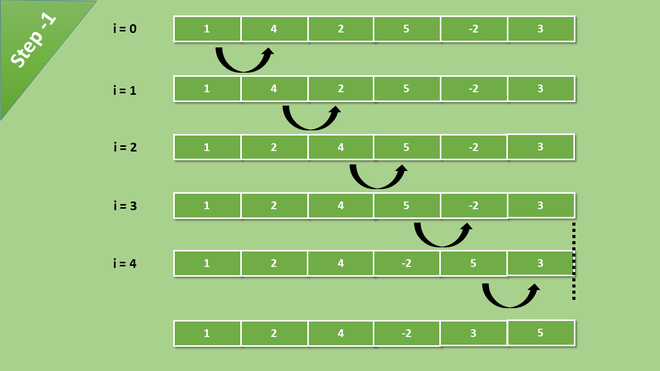
\includegraphics{bubblesort.png}}
    \end{figure}
\end{frame}

\section{Zdroje}
\subsection{Zoznam použitej literatúry}
\begin{frame}{Zoznam použitej literatúry}
    \begin{itemize}
        \setlength\itemsep{1,5em}
        \item \href{https://www.algoritmy.net/article/3/Bubble-sort}{www.algoritmy.net/article/3/Bubble-sort}
        \item \href{https://sk.wikipedia.org/wiki/Bublinkové_triedenie}{sk.wikipedia.org/wiki/Bublinkové\_triedenie}
        \item \href{https://www.programiz.com/dsa/bubble-sort}{www.programiz.com/dsa/bubble-sort}
        \item \href{https://www.w3adda.com/data-structure-tutorial/bubble-sort-algorithm}{www.w3adda.com/data-structure-tutorial}
    \end{itemize}
\end{frame}

\end{document}